% -*- mode: latex; mode: flyspell; ispell-local-dictionary: "en_US"; coding: utf-8; fill-column: 80 -*-

\documentclass{article}

\usepackage[utf8]{inputenc}
\usepackage[english]{babel}

\usepackage{amsmath,amsfonts,amssymb}
\usepackage{fullpage}
\usepackage{verbatim}

\usepackage{tikz,pgfplots}

\pgfplotsset{
  width=150mm,height=100mm,
  major grid style={thin,dotted,color=black!50},
  minor grid style={thin,dotted,color=black!50},
  grid,
  every axis/.append style={
    line width=0.5pt,
    tick style={
      line cap=round,
      thin,
      major tick length=4pt,
      minor tick length=2pt,
    },
  },
  legend cell align=left,
  legend pos=north west,
}

%%%%%%%%%%%%%%%%%%%%%%%%%%%%%%%%%%%%%%%%%%%%%%%%%%%%%%%%%%%%%%%%%%%%%%%%%%%%%%%%

\begin{document}

\title{Laufzeit binäre Suche vs. Mphf-Hashmap}
\author{Tim Tannert}
\maketitle

% IMPORT-DATA stats output/mphf_vs_bs.txt



\begin{center}
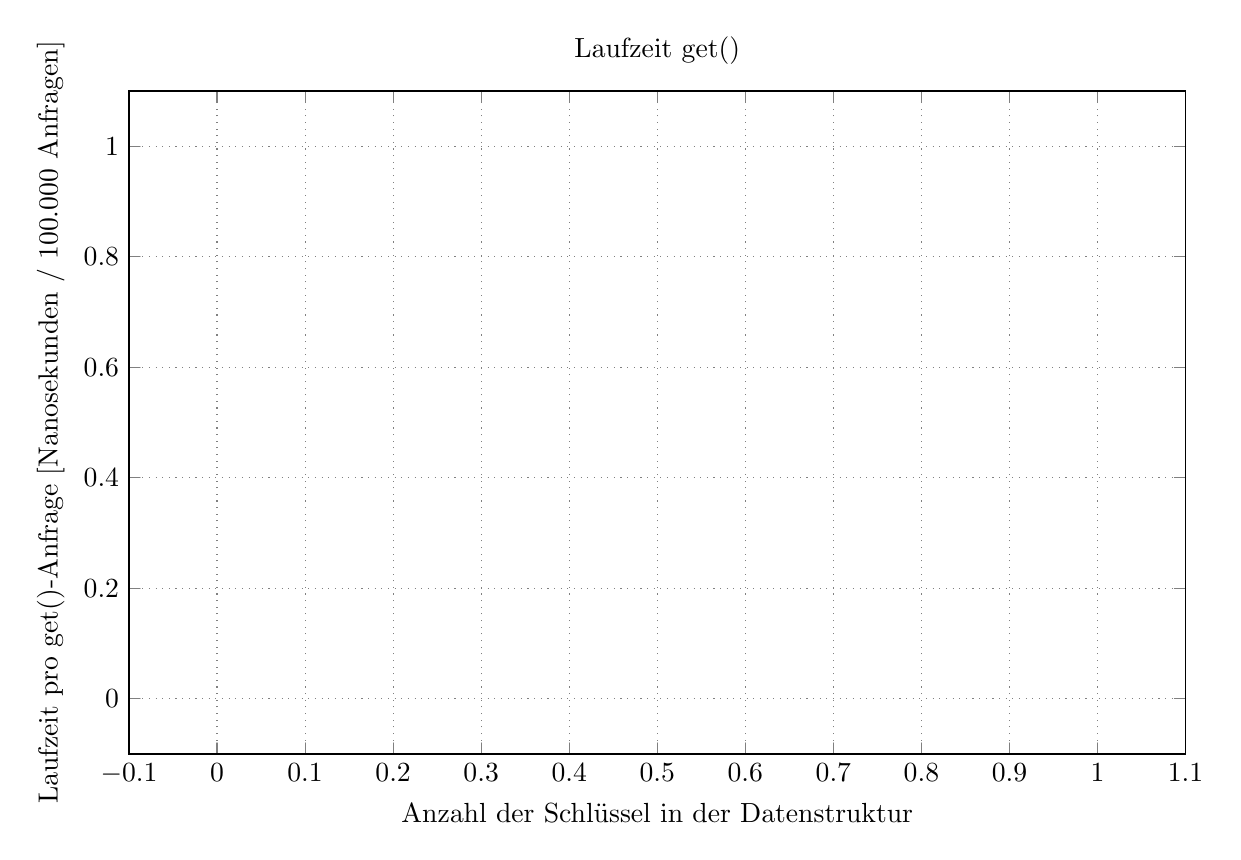
\begin{tikzpicture}
  \begin{axis}[
    title={Laufzeit get()},
    xlabel={Anzahl der Schlüssel in der Datenstruktur},
    ylabel={Laufzeit pro get()-Anfrage [Nanosekunden / 100.000 Anfragen]},
    ]

    %% MULTIPLOT(algo) SELECT size AS x, MEDIAN(time_per_anfrage) AS y, MULTIPLOT
    %% FROM stats GROUP BY MULTIPLOT,x ORDER BY MULTIPLOT,x



  \end{axis}
\end{tikzpicture}
\end{center}





\end{document}
%%%%%%%%%%%%%%%%%%%%%%%%%%%%%%%%%%%%%%%%%%%%%%%%%%%%%%%%%%%%%%%%%%%%%%%%%%%%%%%%
